%Einfache Vorlage fŸr eine mit Latex realisierte Hausarbeit von http://www.studieren-info.de
%Du kannst diese Vorlage fŸr deine Hausarbeit beliebig anpassen%


%-------------------
%Beginn des Kopfbereiches
%-------------------

%Wir verwenden eine DIN-A4-Seite und die Schriftgrš§e 13.
\documentclass[a4paper,13pt]{scrartcl} 


\usepackage{ucs}
\usepackage[utf8x]{inputenc}


%Diese drei Pakete benštigen wir fŸr die Umlaute, Deutsche Silbentrennung etc.
%Apple-Nutzer sollten anstelle von \usepackage[latin1]{inputenc} das Paket \usepackage[applemac]{inputenc} verwenden
%\usepackage[latin1]{inputenc}
\usepackage[ngerman]{babel}
\usepackage[T1]{fontenc}

%Das Paket erzeugt ein anklickbares Verzeichnis in der PDF-Datei.
\usepackage{hyperref}

%Das Paket wird fŸr die anderthalb-zeiligen Zeilenabstand benštigt
\usepackage{setspace}

%EinrŸckung eines neuen Absatzes
\setlength{\parindent}{0em}

%Definition der RŠnder
\usepackage[paper=a4paper,left=30mm,right=30mm,top=30mm,bottom=30mm]{geometry} 

\usepackage{graphicx}

%Abstand der Fu§noten
\deffootnote{1em}{1em}{\textsuperscript{\thefootnotemark\ }}

%Regeln, bis zu welcher Tiefe (section,subsection,subsubsection) †berschriften angezeigt werden sollen (Anzeige der †berschriften im Verzeichnis / Anzeige der Nummerierung)
\setcounter{tocdepth}{3}
\setcounter{secnumdepth}{3}

%-------------------
%Ende des Kopfbereiches
%-------------------




%-------------------
%Hier beginnt der Text deiner Hausarbeit
%-------------------
\begin{document}


%Beginn der Titelseite
\begin{titlepage}
\begin{small}
\vfill {Universität Hamburg \\ Fachbereich Informatik \\ Proseminar Lokale Rechner- und Mobilnetze \\ Sommersemester 2014 \\ Dr. Klaus-Dieter Heidtmann }
\end{small}


\begin{center}
\begin{Large}
\vfill {\textsf{\textbf{
Architekturen und Standards für Rechnernetze und Mobilnetze: 
Wireless Local Area Network
}}}
\end{Large}
\end{center}


\begin{small}
\vfill Juschua Stock \\ David Kirchhausen Monteiro \\ Frederik Wille \\
\today
\end{small}

\end{titlepage}
%Ende der Titelseite


%Inhaltsverzeichnis (aktualisiert sich erst nach dem zweiten Setzen)
\tableofcontents
\thispagestyle{empty}

%Beginn einer neuen Seite
\clearpage

%Anderthalbzeiliger Zeilenabstand ab hier
\onehalfspacing

\pagestyle{plain}


\section{Einleitung}
\subsection{Was ist WLAN?}
Als WLAN (Wireless Local Area Network) bezeichnet man ein lokales Funknetz, das meist einen Standard der IEEE-802.11 Familie implementiert. In vielen Ländern wird für diese Implementationen auch oft der Begriff "WiFi" verwendet (siehe "WlAN, WiFi - Begriffserklärung" im nächsten Kapitel.\\
WLAN ermöglicht heutzutage einen einfachen Zugang zum Internet und hat in sehr vielen Privat- und Berufsstätten Einzug gefunden. Besonders beliebt sind WLAN-Netze in Eigenheimen, wodurch meist auf der gesamten Wohnfläche ein drahtloser Netzwerkkommunikations- und Internetservice bereitgestellt wird. Außerdem sind die meisten Universitäten, Flughäfen, sowie viele Cafés und Restaurants mit sogenannten Hot-Spots ausgestattet, die je nach Bedarf ihr WLAN-Netz der Öffentlichkeit zugänglich machen können.\\
Seit seiner Entstehung wurde WLAN-Netzen immer mehr Beachtung geschenkt und ihre Bedeutung ist stetig gewachsen. Durch diese enorme Popularität und mittlerweile großen Ausbreitung benutzen die meisten Mitglieder unserer Gesellschaft täglich auf die eine oder andere Art WLAN-Netze, sei es mit Mobilgeräten ("Smartphones", Tablets, mobilen Computern) oder mit Tower-Rechnern.
\subsection{Anforderungen}
Typische Anforderungen an WLANs sind beispielsweise ein möglichst hoher Durchsatz an Daten, eine große Anzahl von Klienten (Mobilstationen) und die Interkonnektion mit leitungsgebundenen Netzen. Letztere ermöglicht beispielsweise die beliebte Anbindung an das weltweite Internet. Außerdem sollen die elektromagnetischen Wellen der WLAN-Netze in einem möglichst großen Bereich empfangen werden können und die Mitgliedschaft in einem WLAN-Netz sollte für einen Klienten möglichst stromsparsam möglich sein (um bspw. Handyakkus zu schonen). Des Weiteren sollte der Betrieb möglichst lizenzfrei möglich sein, um insbesondere Privatpersonen das Einrichten eines WLAN-Netzes nicht zu erschweren. Zu guter Letzt sollte garantiert sein, dass das Konfigurieren neu zu integrierender bzw. auszugliedernder Mobilstationen dynamisch passiert und keinen großen Aufwand seitens des Netzbereitstellers fordert.
\subsection{WLAN, WiFi - Begriffserklärung}
Zwischen den Begriffen WLAN und WiFi steckt ein großer Bedeutungsunterschied, der z.B. in Großbrittanien, Kanada und Spanien kaum beachtet wird. WLAN bezeichnet das Netzwerk selber ("Network"), hinter dem Begriff WiFi steckt die WiFi-Alliance. 1999 gegründet, stellt sie seitdem Interoperabilität zwischen Geräten sicher, indem sie Geräte zertifiziert.\\ Konkret funktioniert das folgendermaßen: Hersteller, die sich nach dem Zertifikat für ihr Produkt sehnen, schicken es der Allianz, die das Produkt umfangreich testet. Insbesondere wird (gegen eine Gebühr) getestet, ob es dem entsprechenden IEEE-Standard entspricht und Interoperabilität ermöglicht. Verläuft die Prüfung erfolgreich, darf der Hersteller das Produkt mit dem bekannten WiFi-Logo kennzeichnen.\\
Hintergrund dieser Zertifizierung ist ein, insbesondere in den 90er-Jahren aufkommender Boom der Technologie, der viele Standardaufweichungen, z.B. durch proprietäre Hardware, mit sich zog und Inkompatibilitätsprobleme mit sich zog.
\subsection{Geschichtlicher Hintergrund, ALOHAnet}
Mit zunehmender Bedeutung und Verbreitung von Computern wurden in der zweiten Hälfte des 20. Jahrhunderts Vernetzungsmöglichkeiten zunehmend wichtiger. Auf der Suche nach neuen, insbesondere drahtlosen Mitteln des Informationsaustausches wurde 1970 an der Universität von Hawaii unter der Leitung von Norman Abramson das sogenannte ALOHAnet entwickelt. Es diente ausschließlich Forschungszwecken. Es war das erste Netz, in dem Nutzer über Funkstrecken auf einen Zentralrechner zugreifen konnten.\\
Konkret verband es den Zentralrechner auf der Insel Oahu mit sieben Standorten auf vier Inseln (siehe Abb.1). Später wurde es, mithilfe des Einsatzes von Repeatern, auf weitere Inseln Hawaiis ausgedehnt. Anfänglich konnten Endgeräte nur auf den Großrechner zugreifen, später war es sogar möglich, mit anderen Endgeräten zu kommunizieren.\\
Technisch war ALOHAnet so aufgebaut, dass ein Broadcast- und ein Random-Access-Kanal paralell genutzt wurden. Die Stationen schickten ihre Datenpakete über den Random-Access-Kanal zum Zentralrechner und erhielten nach erfolgreicher Übertragung eine Nachricht des Empfängers über den Broadcast-Kanal. Bei eventueller gleichzeitiger Übertragung von zwei Nachrichten (bzw. Stationen) schlugen beide Versuche fehl und das Senden wurde nach einer zufällig gewählten Zeitspanne wiederholt. Auf diese Weise wurden die Chancen, dass beide Sender beim nächsten Übertragungsversuch wieder eine Kollision erzeugen, minimiert.

%Abbildung 1: Bild mit Inseln und Rechnern
\begin{figure}[ht]
		\centering
	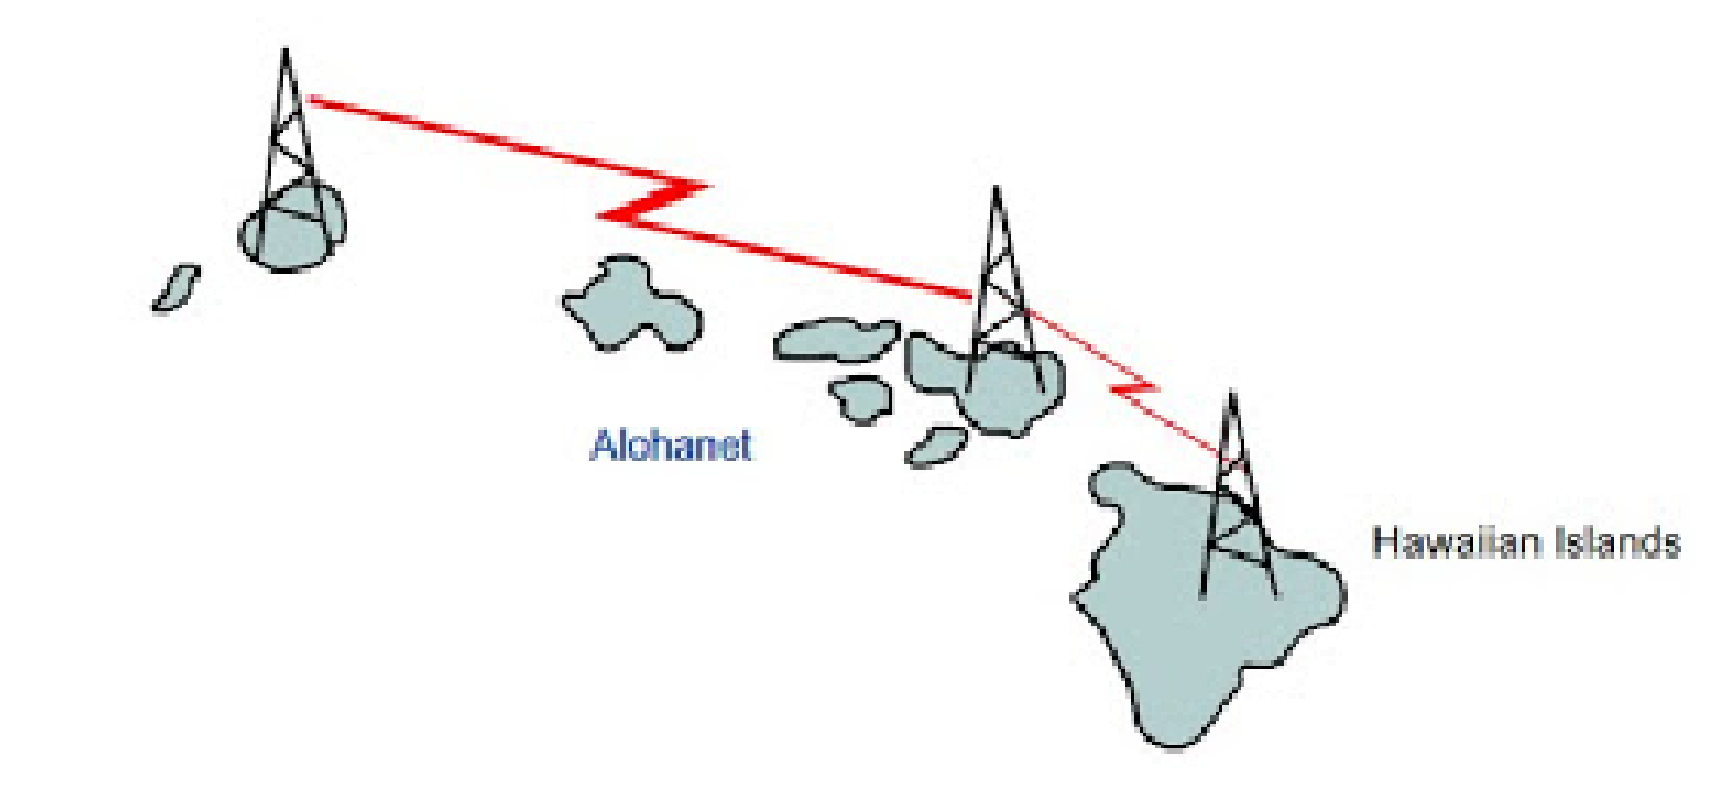
\includegraphics[width=0.5\textwidth]{alohanet.eps}
		\caption{Schematische Darstellung des ALOHAnet}
		\label{fig1}
\end{figure}
\clearpage

\section{Functionalität}

\subsection{Infrastruktur}

shit

\subsection{Ad-Hoc}

noch mehr shit

\section{technische Aspekte}
\subsection{IEEE}
<<<<<<< HEAD
Das Institute of Electrical and Electronics Engineers\footnote{Der volle Name wurde inzwischen fast komplett aufgegeben und wird nur noch für offizielle Dokumente genutzt} ist ein im Jahre 1963 gegründerter Berufsverband von Elektro- und Informationstechnik Ingenieuren. Neben den weitverbreiteten Standards veröffentlicht das IEEE einige sehr angesehene Fachzeitschriften und hält Tagungen. 
Untergliedert ist die IEEE in 
\subsubsection{Unterüberschrift}
foobar
\subsubsection{Unterüberschrift}
asfs
=======
Das Institute of Electrical and Electronics Engineers\footnote{Der volle Name wurde inzwischen fast komplett aufgegeben und wird nur noch für offizielle Dokumente genutzt} ist ein im Jahre 1963 gegründeter Berufsverband von Elektro- und Informationstechnik Ingenieuren. Neben den weitverbreiteten Standards veröffentlicht das IEEE einige sehr angesehene Fachzeitschriften, hält Tagungen und vergibt weltweit angesehene Auszeichnungen. \\
Organisatorisch sind die 425.000 Mitglieder der IEEE in 38 Societies gegliedert, die sich jeweils mit einem bestimmten Teilgebiet beschäftigt und wiederum in über 300 lokale Teilorganisationen unterteilt sind. Als Beispiel gibt es die IEEE Communications Society, die sich unter anderem mit WLAN beschäftigt. Für Gebiete in denen sich die Bereiche mehrerer Societies überschneiden, werden sogenannte Councils gegründet. Für die Entwicklung von Standards sind Komitees zuständig, wie "IEEE 802 LAN/MAN Standards Committee".\\
Um Spenden annehmen und verwalten zu können, wurde 1973 die IEEE Foundation gegründet. Ein Teil dieser Spenden kommen den Auszeichnungsträgern der IEEE zu, während der Rest für Entwicklungs-, Forschungs- und humanitäre Zwecke verwendet wird. \\
Ungefähr 30\% aller Fachzeitschriften in der Elektro- und Informationstechnik wird von der IEEE veröffentlicht, obwohl eine recht strenge Copyright Politik verfolgt wird. Jeder Autor eines in einer dieser veröffentlichen Zeitschriften muss sein gesamtes Copyright an die Organisation abtreten und darf nur für sich und seine Mitarbeiter Kopien behalten. Will der Autor seinen Artikel trotzdem weiter verbreiten, muss er die IEEE für das Copyright bezahlen und die IEEE entsprechend auf der ersten Seite vermerken.
\subsection{IEEE 802}
Die Standardisierungsfamilie 802 beinhaltet wohl die am weitesten verbreiteten Standards. In ihr sind alle Standards zusammengefasst, die sich mit dem Lokal Area Network und dem Metropolitan Area Network befassen. Sie umfasst 25 Standards, wobei zum Beispiel 802.15 das Personal Area Network in 6 Unterstandars geteilt ist. 

\clearpage
\section{Sicherheit}
Um WLAN-Netze zu schützen, existieren diverse Möglichkeiten der Verschlüsselung. 
\subsection{RC4}
RC4 ist eine Stromverschlüsselung, die auch unter ARC4 oder Arcfour bekannt ist. Sie ist eine Marke von RSA Security und geht auf eine Open Source Veröffentlichung von 1994 zurück.\\
Die Verschlüsselungsmethode findet unter anderem in HTTPS, SSH1, WEP und WPA Verwendung.
\subsubsection{Funktionsweise}
Konkret arbeitet RC4 so, dass zunächst eine Zufallsfolge aus einem einmaligem Schlüssel (per "S-Box"\footnote{Bei einer S-Box wird eine m-stellige Binärzahl durch eine n-stellige Binärzahl ersetzt. Sie wird meistens eingesetzt, um die Beziehung zwischen Klar- und Ciphertext zu verwischen (in der Krypto-Fachsprache als "Konfusion" bezeichnet).}) generiert wird. Anschließend daran wird der Klartext Bit für Bit mit der Zufallsfolge XOR-verknüpft. Wichtig hierbei ist, dass die Zufallsfolge auch tatsächlich bei jeder Anwendung neu generiert wird und nicht mehrfach auftritt, da nur so die Sicherheit garantiert werden kann. RC4 ist besonders beliebt, da er einfach in Hard- und Software zu implementieren ist, vergleichsweise effizient berechenbar und dadurch gut kompatibel ist.
\subsubsection{Bedenken}
Da RC4 ein Stromchiffre ist, bietet es keinen Integritätsschutz. Ändert also ein Angreifer ein Bit des Ciphertextes, wird auch das gleiche Bit des Klartextes geändert. 2001 glückte Scott Fluhrer der erste praktische Angriff auf ein RC4-Chiffre. Der Internetaktivist und Spezialist für Computersicherheit Jacob Appelbaum geht davon aus, dass die NSA einen RC4-verschlüsselten Text in Echtzeit brechen kann, diese Meinung wird auch von bspw. Bruce Schneier geteilt.\\
Sowohl die Europäische Agentur für Netz- und Informationssicherheit, als auch das Bundesamt für Sicherheit in der Informationstechnik raten offiziell von der Verwendung von RC4 ab. Die Sicherheit von RC4 ist also alles andere als gegeben.
\subsection{WEP}
Die "Wired Equivalent Privacy" (zu Deutsch wörtlich "Kabelgebundene Äquivalente Privatsphäre") ist die erste, gängige Verschlüsselungsmethode für WLAN-Netzwerke.
\subsubsection{Funktionsweise}
Das WEP-Protokoll verwendet dabei den oben beschriebenen RC4-Algorithmus bei der Erzeugung eines sogenannten Keystreams. Dieser Keystream erhält einen Schlüssel und einen Initialisierungsvektor (IV) als Eingabe. Für jede zu verschlüsselnde Nachricht wird ein neuer IV gebildet und mit einem Schlüssel verknüpft, der allen Basisstationen im Netz bekannt ist (dieses Prinzip ist auch als "Shared Key" bekannt). Zusätzlich zu diesem Keystream wird mittels zyklischer Redundanzprüfung (englisch "Cyclic Redundancy Check", CRC) eine Prüfsumme berechnet und an die Nachricht angehängt. Anschließend wird der verschlüsselten Nachricht der Initialisierungsvektor unverschlüsselt vorangestellt und die Nachricht kann übertragen werden. Der Empfänger der Nachricht kann sich aus der Kombination IV, RC4-Schlüssel und Ciphertext den Klartext errechnen.
\begin{figure}[ht]
		\centering
	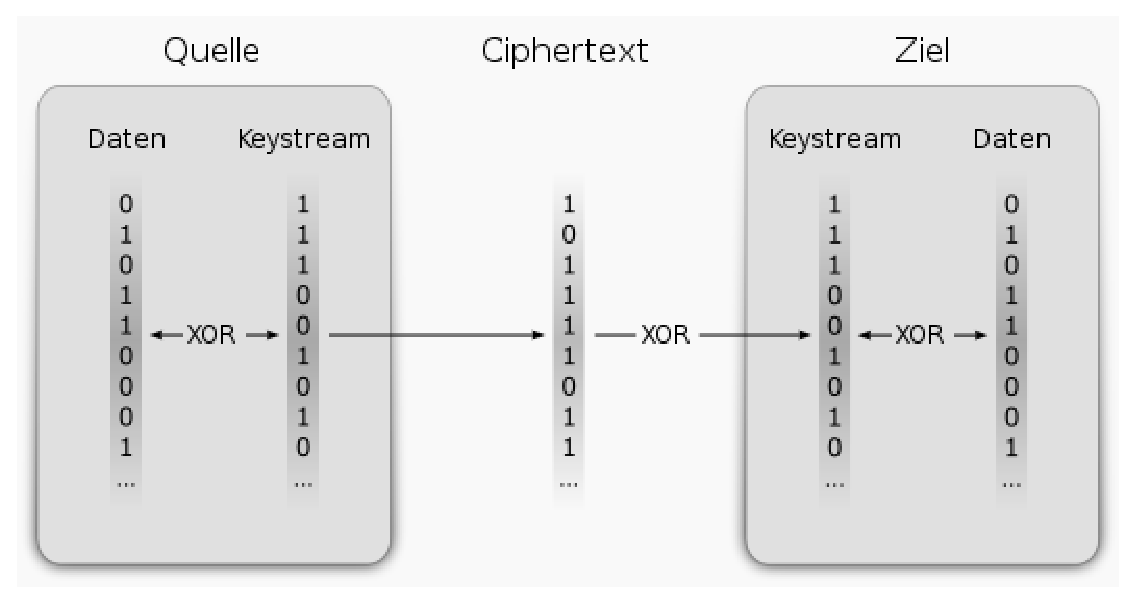
\includegraphics[width=0.4\textwidth]{WEP.eps}
		\caption{Ein Ciphertext wird erstellt und am Zielort entschlüsselt}
		\label{fig2}
\end{figure}
\subsubsection{Das WEP-Datenpaket}
Ein WEP-Datenpaket gliedert sich folgendermaßen: Zusätzlich zu den Nutzdaten steht der 24-Bit-Initialisierungsvektor vor der Nachricht und an der Nachricht steckt, verschlüsselt, die 32-Bit-Prüfsumme ICV (englisch "Integrity Check Value", wörtlich übersetzt "Integritätsprüfsumme").
\begin{figure}[ht]
		\centering
	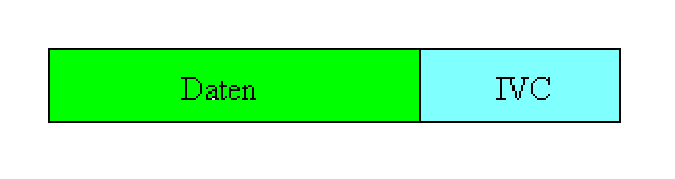
\includegraphics[width=0.5\textwidth]{WEP_DPaket.eps}
		\caption{Der grobe Aufbau eines WEP-Datenpakets}
		\label{fig3}
\end{figure}
\subsubsection{Angriffsmöglichkeiten auf WEP}
Zunächst muss gesagt werden, dass ohne aktive Teilnehmer in einem WEP-Netzwerk die Chancen sehr schlecht stehen, die Verschlüsselung innerhalb vergleichsweise kurzer Zeit zu durchbrechen. Mit Teilnehmern kann man sich allerdings am 24 Bit kurzen Initialisierungsvektor bedienen, der jeder Nachricht unverschlüsselt vorangestellt wird. Ein Angreifer kann mitlauschen, dabei aufzeichnen um sich dann aus mehreren mitgelauschten Vektoren den Schlüssel zu errechnen.\\
%oder Antworten des Acces-Points forcieren, um innerhalb einer Minute genügend Daten für erfolgreichen passiven Angriff zu sammeln
Das folgende Beispiel veranschaulicht diese Methode:
\begin{figure}[ht]
		\centering
	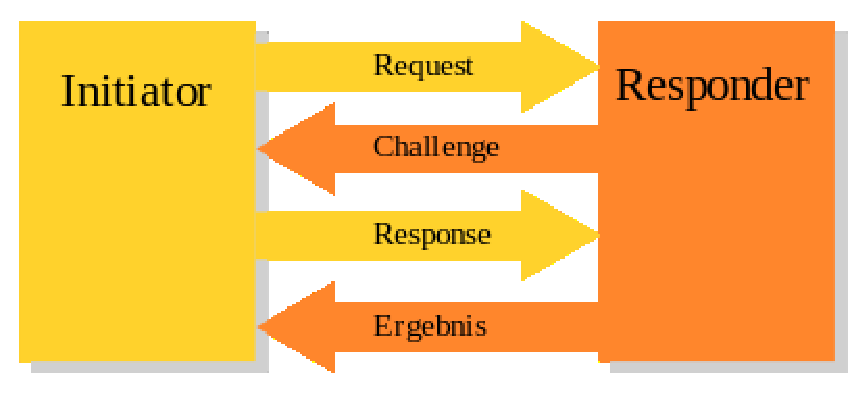
\includegraphics[width=0.4\textwidth]{WEP_Angriff.eps}
		\caption{WEP-Angriffsschema}
		\label{fig3}
\end{figure}\\
Der Server schickt zur Authentifizierung eines Klienten Challenge1, bspw. Zufallszahl eine Zufallszahl, die dieser korrekt verschlüsselt zurück an den Server schicken soll. Der Klient verschlüsselt die "Challenge" und schickt sie als IV1 (Initialisierungsvektor1) + Ciphertext1 zurück.\\
Trudy, die Angreiferin, hat Challenge1, IV1 und Ciphertext1 mitgelauscht.
Mittels XOR kann sie sich nun den Keystream1 errechnen. Da sie den IV1 ebenfalls mitgelauscht hat, hat sie nun eine gültige Kombination Keystream + Initialisierungsvektor. Jetzt kann sie Challenge2 vom Server selber beantworten, nämlich mit dem Paket IV1 + Ciphertext2, wobei der Ciphertext2 mittels Challenge2 XOR Keystream1 berechnet wurde.\\
Trudy schickt dies dem Server und wird erfolgreich authentifiziert.\\
\\
Neben dieser Methode existieren auch andere Angriffstechniken auf WEP-Netzwerke. Angriffsmöglichkeiten: Beispielsweise können mitgehörte Datenpakete entschlüsselt werden, indem man den gesamten Verkehr des Netzwerkes abfängt und einzelne Nachrichten mehrmals leicht modifiziert wieder in das WLAN eingespielt werden. Aus den vom Server geschickten Antworten kann sich nun mittels spezieller Technik der Schlüssel errechnet werden.\\
Eine andere Art des Angriffs ist der "KoreK-Angriff" (benannt nach Pseudonym des Entdeckers). Hierbei wird von einer verschlüsselten Nachricht anfangs nur ein Byte abgeschnitten, durch ein geratenes ersetzt und an den Access Point zurückgeschickt. Akzeptiert der Access Point, hat man richtig geraten und kann nun das nächste Byte raten. Akzeptiert er die teilweise geratenen Nachricht nicht, muss neu geraten und gesendet werden, bis der Access Point akzeptiert. Auf diese Art lässt sich eine ganze Nachricht entschlüsseln um somit den Schlüssel zu errechnen.
\subsection{WPA}
Eine weitere Verschlüsselungsmethode für WLAN-Netzwerke ist der "Wi-Fi Protected Access" WPA (zu Deutsch "Geschützter Wi-Fi Zugriff"). Es handelt sich hierbei um einen sogenannten Pseudostandard, der dem neuen Standard IEEE 802.11i vorweggenommen wurde, da sich WEP als unsicher erwies und sich die Veröffentlichung des gesamten IEE 802.11i-Standards verzögerte. Die Zertifizierung nach WPA begann im Jahre 2003.
\subsubsection{Funktionsweise}
WPA baut großteils auf die Architektur von WEP auf. Allerdings erweitert es dessen Sicherheit, indem es dynamische Schlüssel einführt. Diese basieren auf dem "Temporal Key Integrity Protocol" ("Temporär-Schlüssel-Integritäts-Protokoll")\footnote{TKIP macht pro Paket einen eigenen 128-Bit-Schlüssel. Dabei verwendet den RC4-Algorithmus und die 64-Bit kryptographische Hashfunktion Michael für Message Integrity Checks. Außerdem stellt TKIP sicher, dass jedes Datenpaket mit einem anderen Schlüssel gesichert ist.\\
Das passiert, indem die MAC-Adresse des Klienten und die 48-Bit Sequenznummer mit in den Schlüssel einfließt.}, das 128-Bit-Schlüssel generiert. Dadurch wird die große Sicherheitslücke in WEP großteils übergangen, außerdem wird durch den Message Integrity Check ("Nachrichts-Integritätstest") sichergestellt, dass gesendete Pakete nicht manipuliert von Angreifern in den Verkehr geschleust wurden. Schlägt dieser Test fehl, erkennt der Access Point sofort einen möglichen Angriff auf das Netzwerk.
\subsubsection{Sicherheit}
Wird die gängige Methode des "Pre-Shared-Keys" ("Vorgeteilter Schlüssel") verwendet, also ein Schlüssel ausgetauscht, der allen Klienten bekannt sein muss, kann dieser immer noch durch eine Brute-Force-Attacke oder einen Wörterbuchangriff erraten werden.
\subsubsection{WPA2}
WPA2 ist der Nachfolger von WPA und baut darauf auf. Er implementiert den IEEE 802.11i-Standard und basiert auf dem Advanced Encryption Standard AES ("Erweiterter Verschlüsselungsstandard").
\subsubsection{Advanced Encryption Standard}
Dieser Standard ist eine Blockchiffre, die im Jahre 2000 vom National Institute of Standards and Technology veröffentlicht wurde. Er gilt als vergleichsweise sehr sicher: Erst 10 Jahre nach seiner Veröffentlichung wurde der erste theoretisch interessante (jedoch praktisch irrelevante) Angriff gefunden. Der Algorithmus ist frei verfügbar, kann also in Hard- und Software lizenzfrei implementiert werden.\\
Er basiert auf voneinander unabhängigen Block- und Schlüssellängen von 128 bis 256 Bit. Grob funktioniert die hochkomplizierte Verschlüsselungsmethode folgendermaßen:\\
Jeder zu verschlüsselnde Text wird zunächst in eine 2D-Tabelle mit vier Zeilen geschrieben, deren Zellen je ein Byte groß sind. Somit variiert die Anzahl der Spalten je nach Blockgröße von vier bis acht. Anschließend wird jeder Block nacheinander bestimmten Transformationen unterzogen. Die Besonderheit am AES-Algorithmus ist, dass hierbei verschiedene Teile des Originalschlüssels nacheinander auf den Klartextblock angewendet werden, und nicht wie üblich ein (ganzer) Schlüssel mehrmals verwendet wird.\\
Außerdem benutzt auch AES eine S-Box als Basis der Verschlüsselung. Diese gibt an, wie in jeder Verschlüsselungsrunde jedes Byte eines Blocks durch einen anderen Wert zu ersetzen ist.

\subsection{Gesundheitsaspekte}


\section{Schluss}
afgdfv

%Beginn einer neuen Seite
\clearpage

\section{Literaturverzeichnis}

Musterfrau, Renate: Muster. Frankfurt 2003.


Mustermann, Helmut: Noch ein Muster. Mit einer Einleitung hrsg. von Frank Muster. Frankfurt 2003.

ALOHAnet: http://www.netplanet.org/geschichte/arpa.shtml
http://de.wikipedia.org/wiki/ALOHAnet
Abbildung: Quelle: http://dixland.blogspot.de/2010/09/first-lan-in-world-was-original-version.html

http://de.wikipedia.org/wiki/S-Box
http://de.wikipedia.org/wiki/RC4
http://www.heise.de/security/meldung/NSA-entschluesselt-Webserver-Daten-angeblich-in-Echtzeit-2041383.html
%http://de.wikipedia.org/wiki/Temporal_Key_Integrity_Protocol
%http://de.wikipedia.org/wiki/Wi-Fi_Protected_Access
%http://de.wikipedia.org/wiki/Wired_Equivalent_Privacy

\end{document}
%-------------------
%Hier endet der Text deiner Hausarbeit
%-------------------